\begin{enumerate}[label=\thesection.\arabic*.,ref=\thesection.\theenumi]
\numberwithin{equation}{enumi}

\item
Find the Phase Margin of $G(s)$ in degrees where
\begin{align}
G(s) = \frac{2}{(s+1)(s+2)}
\end{align}
\solution \textbf{Phase Margin}:It is the difference between phase of the system and $-180^{\circ}$ at the gain crossover frequency,(the gain crossover frequency being the frequency at which the open-loop gain first reaches 1).\\
Phase Margin is given by,
\begin{align}
P.M=\phi-\angle G(j\omega)|_{\omega=\omega_{pc}}=\phi+180^{\circ}
\end{align}
where,
\begin{align}
\phi=\angle G(j\omega)|_{\omega=\omega_{gc}}
\label{eq:sol}
\end{align}
$\omega_{pc}$ is the Phase crossover frequency (The frequency at which the phase of open-loop transfer function reaches -180$^{\circ}$).\\
$\omega_{gc}$ is the Gain crossover frequency (The frequency at which the gain of the open-loop transfer fuction reaches 1).\\
Given,

\begin{align}
G(s) = \frac{2}{(s+1)(s+2)} 
\\
G(j\omega)=\frac{1}{(j\omega+1)(j\omega+2)} 
\end{align}
We can find magnitude and phase as

\begin{align}
|G(j\omega)|=\frac{2}{(\sqrt{\omega^2+1})(\sqrt{\omega^2+4})}
\\
\angle G(j\omega)=- tan^{-1}(\omega) - tan^{-1}(\frac{\omega}{2}) \label{eq:solve}
\end{align}

We know that,
Gain in dB = 0 at $\omega=\omega_{gc}$
\begin{align}
20log_{10}|G(j\omega_{gc})|=0 
\\
|G(j\omega_{gc})|=1
\\
\frac{2}{(\sqrt{\omega_{gc}^2+1})(\sqrt{\omega_{gc}^2+4})}=1
\end{align}
Solving we get,
\begin{align}
\omega^2_{gc}(\omega^2_{gc}+5)=0
\\
=> \omega_{gc}=0,+j\sqrt{5},-j\sqrt{5}
\end{align}
As frequency is a real quantity
\\Hence, $\omega_{gc} \neq$ Imaginary
\begin{align}
\therefore  \omega_{gc} =0
\end{align}
From (\ref{eq:solve}) and (\ref{eq:sol})
\begin{align}
\phi= \angle G(j\omega_{gc})= -tan^{-1}(\omega_{gc})-tan^{-1}(\frac{\omega_{gc}}{2})
\end{align}

\begin{align}
=> \phi=0^{\circ}
\\
\therefore P.M=180^{\circ}+0^{\circ}=180^{\circ}
\end{align}

\item
We can verify the above result using phase plot.The following code plots Fig(\ref{fig:ee18btech11017})
\begin{lstlisting}
codes/ee18btech11017.py
\end{lstlisting}
\item
The Phase plot is as shown,
\begin{figure}[!h]
  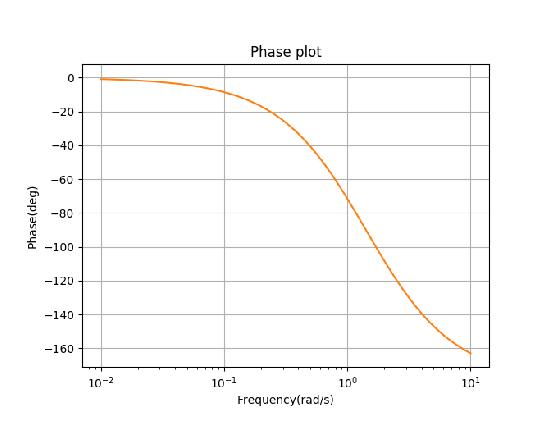
\includegraphics[width=\columnwidth]{./figures/ee18btech11017.eps}
  \caption{}
  \label{fig:ee18btech11017}
\end{figure}
We can observe that at $\omega_{gc}=0$ , $\phi=0^{\circ}$
\\
\begin{align}
\therefore P.M=180^{\circ}
\end{align}
\item
\textbf{Application:} 
Phase margin is measure of stability in closed-loop, dynamic-control systems.(i.e, For stability of a system both gain margin and phase margin should be positive.)
\end{enumerate}
